This is the first sub section that user interacts with. When the user opens the mobile application for the first time details for SignUp is displayed. Then the user enters all the information required for SignUp including all the valid user name and password to create a account. Then an account for the user is created.

\subsection{UI Controller}


\begin{figure}[h!]
	\centering
 	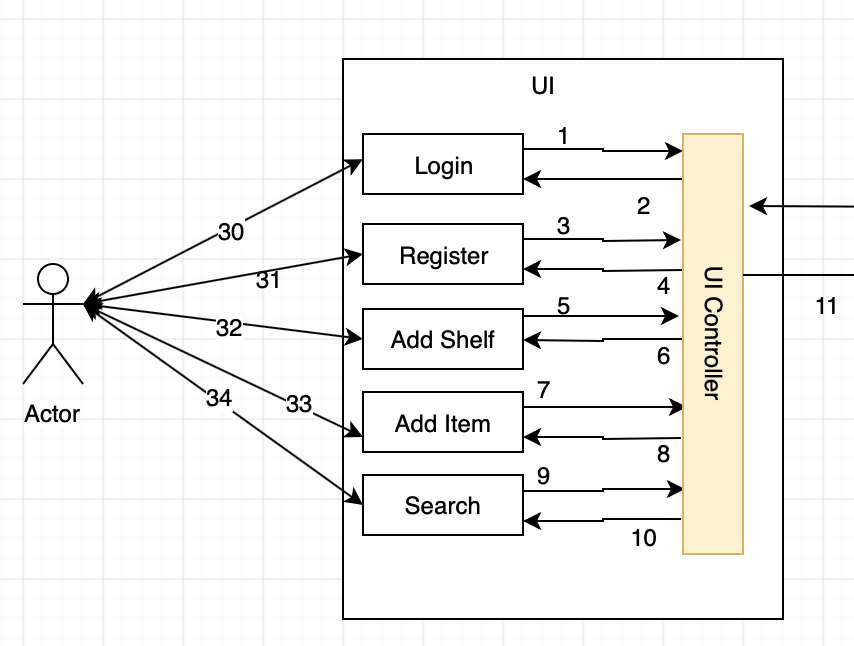
\includegraphics[width=0.60\textwidth]{images/uicontroller}
 \caption{UI Controller description diagram}
\end{figure}

\subsubsection{Assumptions}
Following assumptions are made for this SubSystem:
\begin{itemize}
    \item User select the specific function with some input.
\end{itemize}

\subsubsection{Responsibilities}
Following are the responsibilities of this SubSystem:
\begin{itemize}
    \item To send the user request to Business\_COntroller.
    \item To receive Messages and various images returned by Business\_Controller 
\end{itemize}

\subsubsection{UI\_Controller Subsystem Interfaces}
Each of the inputs and outputs for the subsystem are defined here.

\begin {table}[H]
 
\begin{center}
    \begin{tabular}{ | p{1cm} | p{6cm} | p{3cm} | p{3cm} |}
    \hline
    ID & Description & Inputs & Outputs \\ \hline
    \#1 & Login/UI\_Controller & \pbox{3cm}{Userid \\ Password} & \pbox{3cm}{N/A}  \\ \hline
    \#2 & UI\_Controller/Login & \pbox{3cm}{N/A} & \pbox{3cm}{Success Message \\ Failure Message}  \\ \hline
    \#3 & Register/UI\_Controller & \pbox{3cm}{Userid \\ Password\\User Name \\ Email} & \pbox{3cm}{N/A}  \\ \hline
    \#4 & UI\_Controller/Register & \pbox{3cm}{N/A} & \pbox{3cm}{Success Message \\ Failure Message}  \\ \hline
    \#5 & Add Shelf/UI\_Controller & \pbox{3cm}{Shelf Name \\ #Row\\ #Column \\ Shelf Location} & \pbox{3cm}{N/A}  \\ \hline
    \#6 & UI\_Controller/Add Shelf & \pbox{3cm}{N/A} & \pbox{3cm}{Success Message \\ Failure Message}  \\ \hline
    \#7 & Add Item/UI\_Controller & \pbox{3cm}{Item name \\ BarCode(opt) \\ Quantity\\ Expiration Date(opt)\\ Expiration\_notification(opt)\\ PIN(opt)\\Brewery(if alcohol)\\ Style(if alcohol)} & \pbox{3cm}{N/A}  \\ \hline
    \#8 & UI\_Controller/Add Item & \pbox{3cm}{N/A} & \pbox{3cm}{Success Message \\ Failure Message}  \\ \hline
    \#9 & Search/UI\_Controller & \pbox{3cm}{Item Description/ QR Code} & \pbox{3cm}{N/A}  \\ \hline
    \#10 & UI\_Controller/Search & \pbox{3cm}{N/A} & \pbox{3cm}{Image file}  \\ \hline
    \#11 & UI\_Controller/Business\_Controller & \pbox{3cm}{User input \\ label} & \pbox{3cm}{N/A}  \\ \hline
    \#12 & Business\_Contorller/UI\_Controller & \pbox{3cm}{N/A} & \pbox{3cm}{Success Message \\ Failure Message \\ Item image}  \\ \hline
    \end{tabular}
    \caption {UI\_Controller Subsystem Interfaces}
\end{center}
\end{table}

\subsection{Login}


\begin{figure}[h!]
	\centering
 	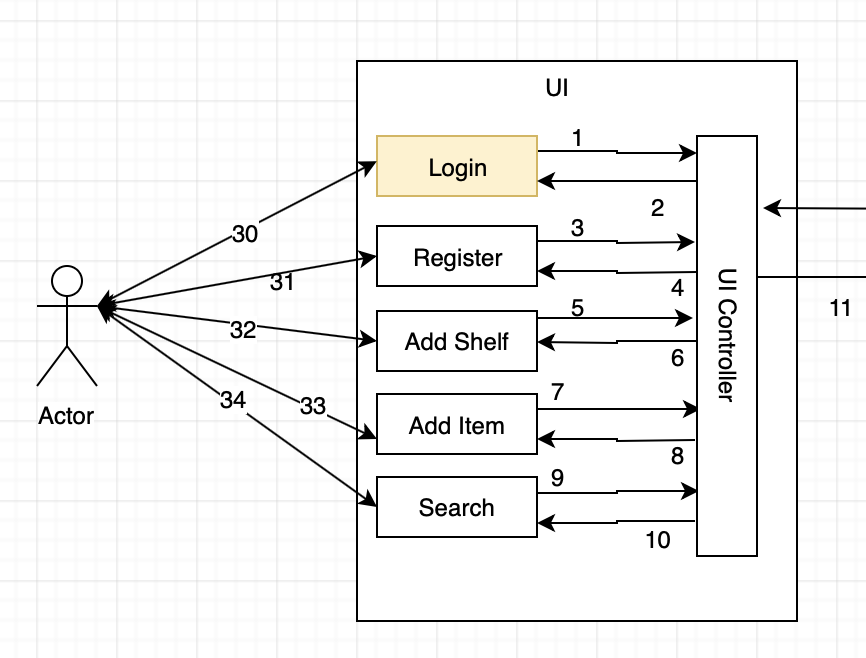
\includegraphics[width=0.60\textwidth]{images/login}
 \caption{Login description diagram}
\end{figure}

\subsubsection{Assumptions}
Following assumptions are made about this SubSystem:
\begin{itemize}
    \item User clicked on the login or signup button in the home screen.
    \item Users cellphone is connected to the internet.
    \item User has a valid Email address.
    \item User provides the password that satisfies the basic password constrain
\end{itemize}

\subsubsection{Responsibilities}
These are the following responsibilities of this subsystem:
\begin{itemize}
    \item Email address must be validated. If Email address doesn’t exist or is not valid, SubSystem must prevent from creating or acessing the account.
    \item If the password doesn’t meet minimum criteria, SubSystem must prevent user form creating account.
\end{itemize}

\subsubsection{Login Subsystem Interfaces}
Each of the inputs and outputs for the subsystem are defined here. An entry for each labelled interface that connects to this subsystem is shown in the table below:

\begin {table}[H]

\begin{center}
    \begin{tabular}{ | p{1cm} | p{6cm} | p{3cm} | p{3cm} |}
    \hline
    ID & Description & Inputs & Outputs \\ \hline
    \#30 & Actor/ Login & \pbox{3cm}{Username \\Password} & \pbox{3cm}{Success message \\ Failure Message}  \\ \hline
    \#1 & Login/UI\_Controller & \pbox{3cm}{Userid \\ Password} & \pbox{3cm}{N/A}  \\ \hline
    \#2 & UI\_Controller/Login & \pbox{3cm}{N/A} & \pbox{3cm}{Success Message \\ Failure Message}  \\ \hline
    \end{tabular}
    \caption {Login Subsystem Interfaces} 
\end{center}
\end{table}

\subsection{Register}


\begin{figure}[h!]
	\centering
 	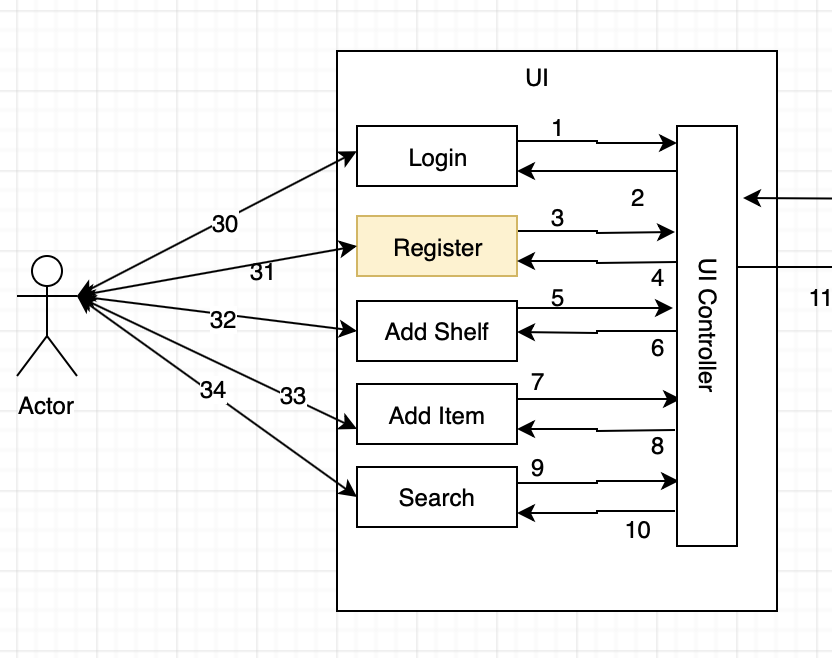
\includegraphics[width=0.60\textwidth]{images/register}
 \caption{Register description diagram}
\end{figure}

\subsubsection{Assumptions}
Following are the assumption of SubSection Email/Password Validation:
\begin{itemize}
    \item User clicked on the register button.
    \item Users cellphone is connected to the internet.
    \item The user inputs all the information in the sign up form.
    \item The User ID and Password input is valid meeting the minimum criteria.
\end{itemize}
\subsubsection{Responsibilities}
Following responsibilities must be carried out by this SubSystem:
\begin{itemize}
    \item Email address, user name and the password is validated. If the provided email address is not valid then user is not allowed to register for the account.
    \item The system must only accept a unique username and a unique email address.
    \item User password must satisfy minimum criteria for the password constrain.
\end{itemize}

\subsubsection{Register Subsystem Interfaces}
Each of the inputs and outputs for the subsystem are defined here. Create a table with an entry for each labelled interface that connects to this subsystem. For each entry, describe any incoming and outgoing data elements will pass through this interface.

\begin {table}[H]

\begin{center}
    \begin{tabular}{ | p{1cm} | p{6cm} | p{3cm} | p{3cm} |}
    \hline
    ID & Description & Inputs & Outputs \\ \hline
    \#31 & Actor/Register & \pbox{3cm}{Username\\Password\\Email} & \pbox{3cm}{Success Message \\ Failure Message}  \\ \hline
    \#3 & Register/UI\_Controller & \pbox{3cm}{Userid \\ Password\\User Name \\ Email} & \pbox{3cm}{N/A}  \\ \hline
    \#4 & UI\_Controller/Register & \pbox{3cm}{N/A} & \pbox{3cm}{Success Message \\ Failure Message}  \\ \hline
    \end{tabular}
    \caption {Register Subsystem Interfaces} 
\end{center}
\end{table}


\subsection{Add Shelf}


\begin{figure}[h!]
	\centering
 	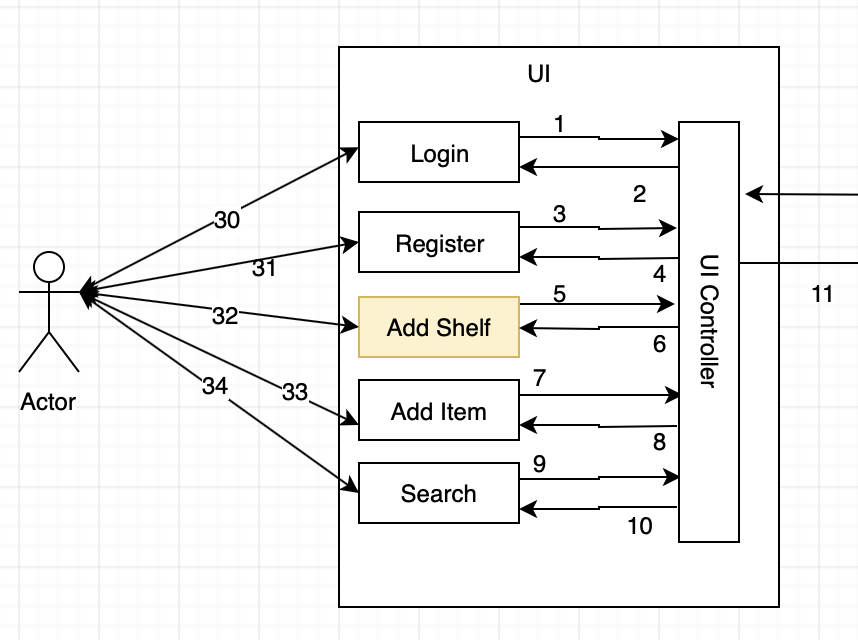
\includegraphics[width=0.60\textwidth]{images/addshelf}

 \caption{Adding Shelf description diagram}

\end{figure}

\subsubsection{Assumptions}
Following assumptions are made about this SubSystem:
\begin{itemize}
    \item User clicked on the add shelf button
    \item Users cellphone is connected to the internet.
    \item User inputs all the information required to create a new shelf
    \item User inputs a valid measurement dimensions.
\end{itemize}

\subsubsection{Responsibilities}
These are the following responsibilities of this subsystem:
\begin{itemize}
    \item The system validate the measurement.
\end{itemize}

\subsubsection{Add Shelf Subsystem Interfaces}
Each of the inputs and outputs for the Add shelf subsystem are defined here.

\begin {table}[H]

\begin{center}
    \begin{tabular}{ | p{1cm} | p{6cm} | p{3cm} | p{3cm} |}
    \hline
    ID & Description & Inputs & Outputs \\ \hline
    \#32 & Actor/Add shelf & \pbox{3cm}{Shelf Name \\ #Row\\ #Column \\ Shelf Location} & \pbox{3cm}{Success Message \\ Failure Message} \\ \hline
   \#5 & Add Shelf/UI\_Controller & \pbox{3cm}{Shelf Name \\ #Row\\ #Column \\ Shelf Location} & \pbox{3cm}{N/A}  \\ \hline
    \#6 & UI\_Controller/Add Shelf & \pbox{3cm}{N/A} & \pbox{3cm}{Success Message \\ Failure Message}  \\ \hline
    \end{tabular}
    \caption {Add Shelf Subsystem Interfaces} 
\end{center}
\end{table}

\subsection{Add Item}
Add Item allows the user to add the items with the description of its different attributes. Attributes like name of product, brand name, manufacture date, best by date and size of product.


\begin{figure}[h!]
	\centering
 	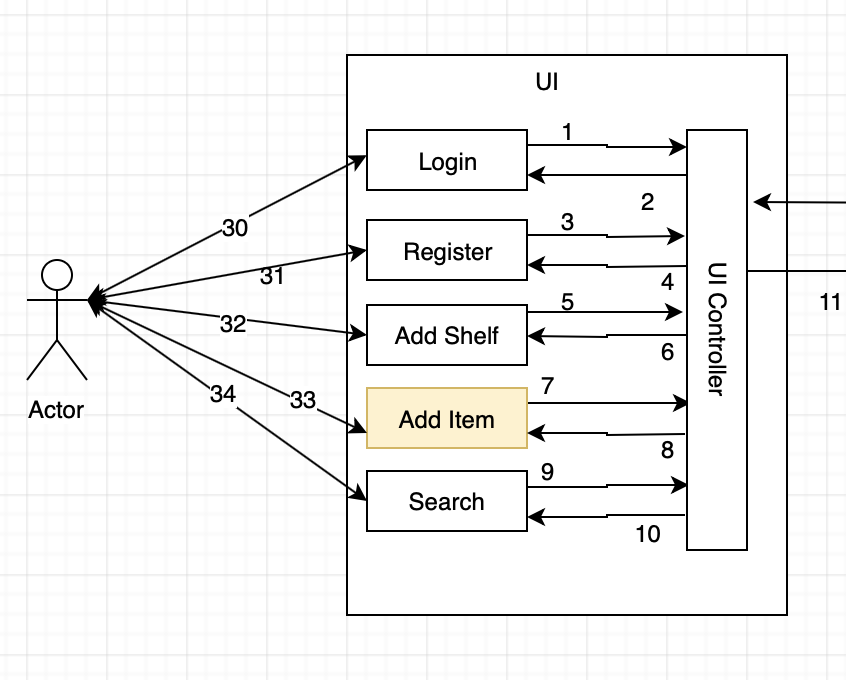
\includegraphics[width=0.60\textwidth]{images/additem}

 \caption{Adding items description diagram}

\end{figure}

\subsubsection{Assumptions}
Following assumptions are made about this SubSystem:
\begin{itemize}
    \item User clicked on add item button
    \item Users cell phone is connected to the internet
    \item User input detailed description about the item.
\end{itemize}

\subsubsection{Responsibilities}
These are the following responsibilities of this subsystem:
\begin{itemize}
    \item The system must get the detailed information from the user and send it to the UI Controller.
\end{itemize}

\subsubsection{Add Item Subsystem Interfaces}
Each of the inputs and outputs for the subsystem are defined here. Create a table with an entry for each labelled interface that connects to this subsystem. For each entry, describe any incoming and outgoing data elements will pass through this interface.

\begin {table}[H]

\begin{center}
    \begin{tabular}{ | p{1cm} | p{6cm} | p{3cm} | p{3cm} |}
    \hline
    ID & Description & Inputs & Outputs \\ \hline
    \#33 & Actor/ Add Item & \pbox{3cm}{Item name \\ BarCode(opt) \\ Quantity\\ Expiration Date(opt)\\ Expiration\_notification(opt)\\ PIN(opt)\\Brewery(if alcohol)\\ Style(if alcohol)} & \pbox{3cm}{Success Message \\ Failure Message}  \\ \hline
    \#7 & Add Item/UI\_Controller & \pbox{3cm}{Item name \\ BarCode(opt) \\ Quantity\\ Expiration Date(opt)\\ Expiration\_notification(opt)\\ PIN(opt)\\Brewery(if alcohol)\\ Style(if alcohol)} & \pbox{3cm}{N/A}  \\ \hline
    \#8 & UI\_Controller/Add Item & \pbox{3cm}{N/A} & \pbox{3cm}{Success Message \\ Failure Message}  \\ \hline
    \end{tabular}
    \caption {Add Item Subsystem Interfacess} 
\end{center}
\end{table}

\subsection{Search}


\begin{figure}[h!]
	\centering
 	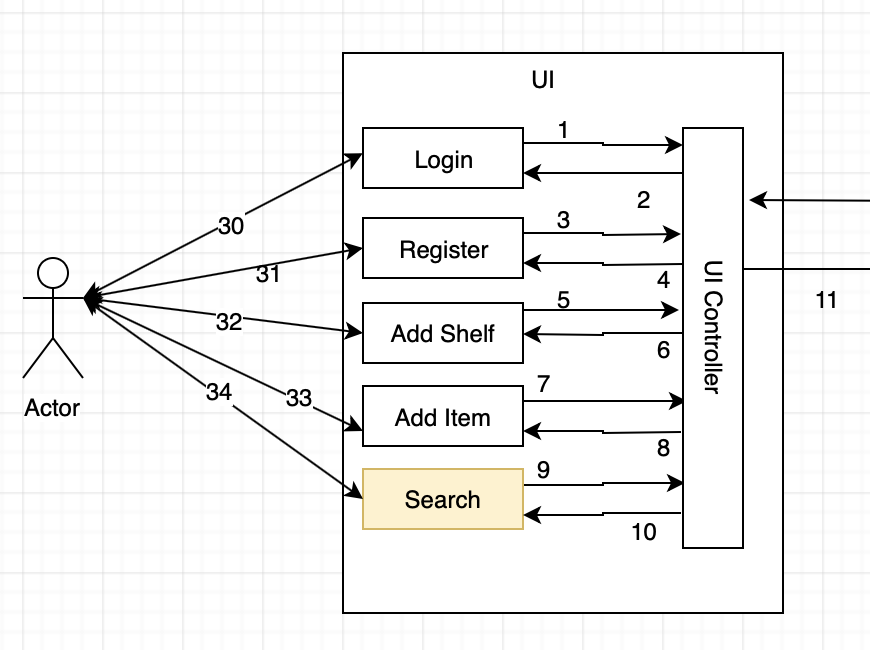
\includegraphics[width=0.60\textwidth]{images/search}
 \caption{searching item description diagram}
\end{figure}

\subsubsection{Assumptions}
Following assumptions are made about this SubSystem:
\begin{itemize}
    \item User clicked on the search button
    \item Users cell phone is connected to the internet
    \item User search for the item with either bar code or manually. If search is with the bar code camera is accessed to scan the bar code and if the search is manual then a text entry field is available.
\end{itemize}

\subsubsection{Responsibilities}
These are the following responsibilities of this subsystem:
\begin{itemize}
    \item The system should be able to get the data from user and send it to the UI Controller.
\end{itemize}

\subsubsection{Search Subsystem Interfaces}
Each of the inputs and outputs for the subsystem are defined here. Create a table with an entry for each labelled interface that connects to this subsystem. For each entry, describe any incoming and outgoing data elements will pass through this interface.

\begin {table}[H]

\begin{center}
    \begin{tabular}{ | p{1cm} | p{6cm} | p{3cm} | p{3cm} |}
    \hline
    ID & Description & Inputs & Outputs \\ \hline
    \#34 & Actor/Search & \pbox{3cm}{Item Description/ QR Code} & \pbox{3cm}{Image file}  \\ \hline
   \#9 & Search/UI\_Controller & \pbox{3cm}{Item Description/ QR Code} & \pbox{3cm}{N/A}  \\ \hline
    \#10 & UI\_Controller/Search & \pbox{3cm}{N/A} & \pbox{3cm}{Image file}  \\ \hline
    \end{tabular}
    \caption {Search Subsystem Interfaces} 
\end{center}
\end{table}

